% Options for packages loaded elsewhere
\PassOptionsToPackage{unicode}{hyperref}
\PassOptionsToPackage{hyphens}{url}
\PassOptionsToPackage{dvipsnames,svgnames,x11names}{xcolor}
%
\documentclass[
  10pt,
  a4paper,
]{article}
\usepackage{amsmath,amssymb}
\usepackage{setspace}
\usepackage{iftex}
\ifPDFTeX
  \usepackage[T1]{fontenc}
  \usepackage[utf8]{inputenc}
  \usepackage{textcomp} % provide euro and other symbols
\else % if luatex or xetex
  \usepackage{unicode-math} % this also loads fontspec
  \defaultfontfeatures{Scale=MatchLowercase}
  \defaultfontfeatures[\rmfamily]{Ligatures=TeX,Scale=1}
\fi
\usepackage{lmodern}
\ifPDFTeX\else
  % xetex/luatex font selection
  \setmainfont[]{Latin Modern Roman}
  \setsansfont[]{Latin Modern Sans}
  \setmonofont[]{DejaVu Sans Mono}
\fi
% Use upquote if available, for straight quotes in verbatim environments
\IfFileExists{upquote.sty}{\usepackage{upquote}}{}
\IfFileExists{microtype.sty}{% use microtype if available
  \usepackage[]{microtype}
  \UseMicrotypeSet[protrusion]{basicmath} % disable protrusion for tt fonts
}{}
\makeatletter
\@ifundefined{KOMAClassName}{% if non-KOMA class
  \IfFileExists{parskip.sty}{%
    \usepackage{parskip}
  }{% else
    \setlength{\parindent}{0pt}
    \setlength{\parskip}{6pt plus 2pt minus 1pt}}
}{% if KOMA class
  \KOMAoptions{parskip=half}}
\makeatother
\usepackage{xcolor}
\usepackage[margin=23mm]{geometry}
\usepackage{color}
\usepackage{fancyvrb}
\newcommand{\VerbBar}{|}
\newcommand{\VERB}{\Verb[commandchars=\\\{\}]}
\DefineVerbatimEnvironment{Highlighting}{Verbatim}{commandchars=\\\{\}}
% Add ',fontsize=\small' for more characters per line
\newenvironment{Shaded}{}{}
\newcommand{\AlertTok}[1]{\textcolor[rgb]{1.00,0.00,0.00}{\textbf{#1}}}
\newcommand{\AnnotationTok}[1]{\textcolor[rgb]{0.38,0.63,0.69}{\textbf{\textit{#1}}}}
\newcommand{\AttributeTok}[1]{\textcolor[rgb]{0.49,0.56,0.16}{#1}}
\newcommand{\BaseNTok}[1]{\textcolor[rgb]{0.25,0.63,0.44}{#1}}
\newcommand{\BuiltInTok}[1]{\textcolor[rgb]{0.00,0.50,0.00}{#1}}
\newcommand{\CharTok}[1]{\textcolor[rgb]{0.25,0.44,0.63}{#1}}
\newcommand{\CommentTok}[1]{\textcolor[rgb]{0.38,0.63,0.69}{\textit{#1}}}
\newcommand{\CommentVarTok}[1]{\textcolor[rgb]{0.38,0.63,0.69}{\textbf{\textit{#1}}}}
\newcommand{\ConstantTok}[1]{\textcolor[rgb]{0.53,0.00,0.00}{#1}}
\newcommand{\ControlFlowTok}[1]{\textcolor[rgb]{0.00,0.44,0.13}{\textbf{#1}}}
\newcommand{\DataTypeTok}[1]{\textcolor[rgb]{0.56,0.13,0.00}{#1}}
\newcommand{\DecValTok}[1]{\textcolor[rgb]{0.25,0.63,0.44}{#1}}
\newcommand{\DocumentationTok}[1]{\textcolor[rgb]{0.73,0.13,0.13}{\textit{#1}}}
\newcommand{\ErrorTok}[1]{\textcolor[rgb]{1.00,0.00,0.00}{\textbf{#1}}}
\newcommand{\ExtensionTok}[1]{#1}
\newcommand{\FloatTok}[1]{\textcolor[rgb]{0.25,0.63,0.44}{#1}}
\newcommand{\FunctionTok}[1]{\textcolor[rgb]{0.02,0.16,0.49}{#1}}
\newcommand{\ImportTok}[1]{\textcolor[rgb]{0.00,0.50,0.00}{\textbf{#1}}}
\newcommand{\InformationTok}[1]{\textcolor[rgb]{0.38,0.63,0.69}{\textbf{\textit{#1}}}}
\newcommand{\KeywordTok}[1]{\textcolor[rgb]{0.00,0.44,0.13}{\textbf{#1}}}
\newcommand{\NormalTok}[1]{#1}
\newcommand{\OperatorTok}[1]{\textcolor[rgb]{0.40,0.40,0.40}{#1}}
\newcommand{\OtherTok}[1]{\textcolor[rgb]{0.00,0.44,0.13}{#1}}
\newcommand{\PreprocessorTok}[1]{\textcolor[rgb]{0.74,0.48,0.00}{#1}}
\newcommand{\RegionMarkerTok}[1]{#1}
\newcommand{\SpecialCharTok}[1]{\textcolor[rgb]{0.25,0.44,0.63}{#1}}
\newcommand{\SpecialStringTok}[1]{\textcolor[rgb]{0.73,0.40,0.53}{#1}}
\newcommand{\StringTok}[1]{\textcolor[rgb]{0.25,0.44,0.63}{#1}}
\newcommand{\VariableTok}[1]{\textcolor[rgb]{0.10,0.09,0.49}{#1}}
\newcommand{\VerbatimStringTok}[1]{\textcolor[rgb]{0.25,0.44,0.63}{#1}}
\newcommand{\WarningTok}[1]{\textcolor[rgb]{0.38,0.63,0.69}{\textbf{\textit{#1}}}}
\usepackage{longtable,booktabs,array}
\usepackage{calc} % for calculating minipage widths
% Correct order of tables after \paragraph or \subparagraph
\usepackage{etoolbox}
\makeatletter
\patchcmd\longtable{\par}{\if@noskipsec\mbox{}\fi\par}{}{}
\makeatother
% Allow footnotes in longtable head/foot
\IfFileExists{footnotehyper.sty}{\usepackage{footnotehyper}}{\usepackage{footnote}}
\makesavenoteenv{longtable}
\setlength{\emergencystretch}{3em} % prevent overfull lines
\providecommand{\tightlist}{%
  \setlength{\itemsep}{0pt}\setlength{\parskip}{0pt}}
\setcounter{secnumdepth}{-\maxdimen} % remove section numbering
\usepackage{tikz}
\usetikzlibrary{arrows.meta}
\usepackage{pdflscape}
\usepackage{xurl}
\usepackage{fancyhdr}
\usepackage{needspace}
\usepackage{etoolbox}
\usepackage{fvextra}
\fvset{breaklines=true,fontsize=\small}
\pagestyle{fancy}
\fancyhf{}
\fancyhead[L]{\footnotesize\sffamily The Compact Post-Quantum KEM Trade-Off}
\fancyhead[R]{\footnotesize\sffamily Kaya / Moser}
\fancyfoot[C]{\small\thepage}
\setlength{\headheight}{14pt}
\renewcommand{\headrulewidth}{0.3pt}
\renewcommand{\footrulewidth}{0pt}
\setlength{\emergencystretch}{3em}
\widowpenalty=10000
\clubpenalty=10000
\raggedbottom
\pretocmd{\section}{\Needspace{6\baselineskip}}{}{}
\AtBeginDocument{\hypersetup{hidelinks,pdftitle={The Compact Post-Quantum KEM Trade-Off},pdfauthor={Yusuf Kaya; Jan Moser},pdfsubject={A falsification-led investigation of compact post-quantum key encapsulation},pdfkeywords={post-quantum cryptography, KEM, ML-KEM, NTRU, HQC, BIKE, isogenies, quantum cryptanalysis},pdfcreator={XeLaTeX / Pandoc},pdfinfo={Repository={https://github.com/kasumigaokasama/compact-pq-kem-tradeoff}}}}
\ifLuaTeX
  \usepackage{selnolig}  % disable illegal ligatures
\fi
\IfFileExists{bookmark.sty}{\usepackage{bookmark}}{\usepackage{hyperref}}
\IfFileExists{xurl.sty}{\usepackage{xurl}}{} % add URL line breaks if available
\urlstyle{same}
\hypersetup{
  colorlinks=true,
  linkcolor={Maroon},
  filecolor={Maroon},
  citecolor={Blue},
  urlcolor={Blue},
  pdfcreator={LaTeX via pandoc}}

\author{}
\date{}

\begin{document}

\setstretch{1.08}
\begin{titlepage}
\thispagestyle{empty}
\vspace*{1.4cm}
{\sffamily\small INDEPENDENT RESEARCH PROJECT\par}
\vspace{1.2cm}
{\sffamily\bfseries\fontsize{30}{35}\selectfont The Compact\\Post-Quantum\\KEM Trade-Off\par}
\vspace{.9cm}
{\Large\raggedright A Falsification-Led Investigation of Compactness, Security, Correctness and Maturity in Post-Quantum Key Encapsulation\par}
\vspace{1.4cm}
{\Large Yusuf Kaya $\cdot$ Jan Moser\par}
\vspace{.35cm}
Independent Research Project\par
\vfill
\hrule\vspace{.5cm}
\textsf{Final Technical Assessment}\\[5pt]
Evidence cutoff: 27 September 2026\\[16pt]
\small Repository:\\
\url{https://github.com/kasumigaokasama/compact-pq-kem-tradeoff}\\[16pt]
Copyright 2026 Yusuf Kaya and Jan Moser.\\
Paper and original figures: CC BY 4.0.\\
\url{https://creativecommons.org/licenses/by/4.0/}
\end{titlepage}
\pagenumbering{roman}

\hypertarget{abstract}{%
\subsection{Abstract}\label{abstract}}

We investigated why a post-quantum key-encapsulation mechanism (KEM)
with substantially less communication than mature alternatives, modest
computation and memory, simple constant-time implementation, and a
credible chosen-ciphertext security argument is difficult to obtain
simultaneously. A broad initial survey was followed by compact-NTRU,
quasi-cyclic Hamming-decoding, and class-group/isogeny-action audits.
The project reproduced selected DAWN packing and failure-\emph{model}
arithmetic, calculated representation bounds and QC support entropies,
and attempted to falsify candidate compression mechanisms. Its decisive
negative result is scoped: \textbf{no investigated mechanism passed all
project gates for constructing a new compact KEM}. Existing compact
designs exploit considerable obvious encoding slack; larger gains
generally alter the decoder, assumption stack, quantum attack surface,
or proof and validation burden. This is an empirical conclusion about
the investigated families through the cutoff date, not an optimality
theorem or a claim that future compact KEMs are impossible. The
scientifically appropriate outcome is to terminate candidate
construction while recording precise triggers for reopening the
question.

\textbf{Keywords:} post-quantum cryptography; KEM; ML-KEM; NTRU; QC
decoding; group actions; quantum cryptanalysis; decryption failures.

\hypertarget{research-contributions}{%
\subsection{Research Contributions}\label{research-contributions}}

\begin{enumerate}
\def\labelenumi{\arabic{enumi}.}
\tightlist
\item
  Cross-family investigation of communication, security, correctness,
  implementation and maturity trade-offs.
\item
  Independent reproduction of selected DAWN packing arithmetic and
  same-alphabet representation bounds.
\item
  Independent reproduction of published DAWN DFR-model arithmetic, with
  an explicit boundary to real correlated DFR assurance.
\item
  Information-theoretic representation analysis for selected NTRU and QC
  constructions.
\item
  Falsification-led NTRU, QC-Hamming and group-action audits, including
  the distinction between compact NIKE and complete IND-CCA
  communication.
\item
  Evidence-specific triggers for reopening terminated research branches.
\end{enumerate}

These are project contributions; peer-reviewed novelty is not claimed.

\hypertarget{evidence-confidence-legend}{%
\subsection{Evidence / Confidence
Legend}\label{evidence-confidence-legend}}

\begin{longtable}[]{@{}
  >{\raggedright\arraybackslash}p{(\columnwidth - 2\tabcolsep) * \real{0.5000}}
  >{\raggedright\arraybackslash}p{(\columnwidth - 2\tabcolsep) * \real{0.5000}}@{}}
\toprule\noalign{}
\begin{minipage}[b]{\linewidth}\raggedright
Label
\end{minipage} & \begin{minipage}[b]{\linewidth}\raggedright
Meaning
\end{minipage} \\
\midrule\noalign{}
\endhead
\bottomrule\noalign{}
\endlastfoot
ESTABLISHED & Definition, exact standard encoding or documented theorem
/ attack under its stated hypotheses. \\
STRONGLY SUPPORTED & Convergent evidence for a conditional
assessment. \\
PROJECT-REPRODUCED & Project calculation of an explicitly specified
model. \\
PLAUSIBLE & Argued extrapolation or inference. \\
SPECULATIVE & Proposed mechanism without adequate validation. \\
UNKNOWN & Required evidence is absent. \\
\end{longtable}

ESTABLISHED does not mean perfectly secure. UNKNOWN does not mean
insecure. Evidence roles remain PROJECT-DERIVED RESULT, EXTERNAL
LITERATURE RESULT, INFERENCE and OPEN QUESTION; AUTHOR CLAIM remains
attributed.

\clearpage\tableofcontents\clearpage\listoffigures\clearpage
\pagenumbering{arabic}

\hypertarget{research-question-and-original-objective}{%
\subsection{1. Research question and original
objective}\label{research-question-and-original-objective}}

The initial goal was a public-key primitive with approximately 128-bit
post-quantum strength, short \textbf{public key and ciphertext
together}, low CPU/RAM/stack cost, manageable constant-time
implementation, and a defensible IND-CCA path based on a
well-articulated average-case hard problem. The earlier informal
ambition of being ``unbreakable after quantum computers'' cannot be a
cryptographic guarantee. Security instead means resistance to specified
classical and quantum attacks at explicit time, memory, query, depth and
circuit costs under a stated assumption, security game and parameter
distribution.

The central question is why this conjunction resists straightforward
construction. A short encoding is only one coordinate; an attack may
exploit the very algebra that made it short. An efficient secret decoder
may make rare failures and chosen-ciphertext behavior the dominant
issue. A one-curve key exchange is not automatically an IND-CCA KEM.

\hypertarget{methodology-and-evidence-categories}{%
\subsection{2. Methodology and evidence
categories}\label{methodology-and-evidence-categories}}

\textbf{PROJECT-DERIVED RESULT} denotes calculations, experiments or
branch decisions made in this project. \textbf{EXTERNAL LITERATURE
RESULT} denotes a standard, paper, specification or attack with its
actual scope. \textbf{INFERENCE} denotes an argument that combines those
pieces but was not proved. \textbf{OPEN QUESTION} marks a missing
theorem, source, estimator run or measurement. Confidence labels are
\textbf{ESTABLISHED} for definitions, exact standard byte encodings or
documented theorem/attack within their hypotheses; \textbf{STRONGLY
SUPPORTED} for convergent but conditional evidence;
\textbf{PROJECT-REPRODUCED} for our model calculations;
\textbf{PLAUSIBLE} for argued extrapolations; \textbf{SPECULATIVE} for
proposed mechanisms; and \textbf{UNKNOWN} where the required evidence is
absent.

The project sequence was landscape triage → compact NTRU review →
reproducibility and falsification → NTRU decision → QC-Hamming audit →
group-action audit → this synthesis. Phase 2B explicitly recorded a
\emph{partial} validation, not a completed source freeze. Phase 2C
formally returned \textbf{INSUFFICIENT EVIDENCE --- PRIMARY VALIDATION
STILL IMPOSSIBLE}, while also answering \textbf{NO} to constructing a
new NTRU candidate. Phase 3 and 4A returned NO-GO under their respective
construction gates. These distinct verdicts must not be flattened into
``we broke every candidate.'' Internal source anchors are listed in
Appendix D and \texttt{PROJECT\_TIMELINE.md}.

External time-sensitive facts were checked against NIST, author
specifications, ePrint records and author communications through the
cutoff date. An author's size or speed claim is attributed rather than
silently upgraded to independent verification. We did not run a fresh
full lattice or quantum ISD estimator.

\begin{figure}[htbp]
\centering
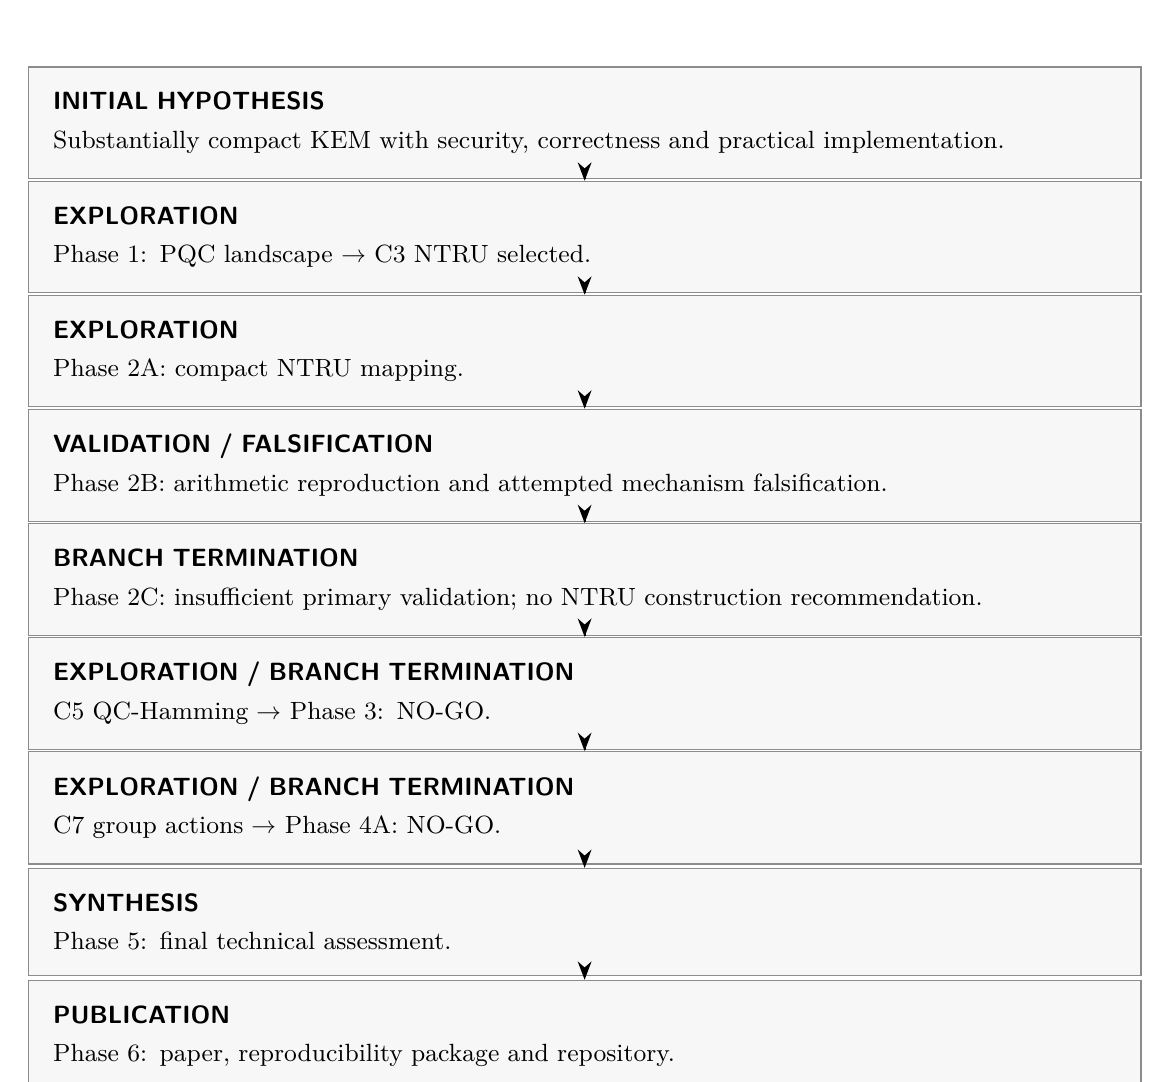
\begin{tikzpicture}[every node/.style={font=\small,align=left},box/.style={draw=black!45,fill=black!3,inner sep=9pt,text width=13.5cm}]
\node[box] (n0) at (0,0.0) {\textsf{\textbf{INITIAL HYPOTHESIS}}\\[3pt]Substantially compact KEM with security, correctness and practical implementation.};
\node[box] (n1) at (0,-1.45) {\textsf{\textbf{EXPLORATION}}\\[3pt]Phase 1: PQC landscape $\rightarrow$ C3 NTRU selected.};
\draw[-{Stealth},thick] (n0.south) -- (n1.north);
\node[box] (n2) at (0,-2.9) {\textsf{\textbf{EXPLORATION}}\\[3pt]Phase 2A: compact NTRU mapping.};
\draw[-{Stealth},thick] (n1.south) -- (n2.north);
\node[box] (n3) at (0,-4.35) {\textsf{\textbf{VALIDATION / FALSIFICATION}}\\[3pt]Phase 2B: arithmetic reproduction and attempted mechanism falsification.};
\draw[-{Stealth},thick] (n2.south) -- (n3.north);
\node[box] (n4) at (0,-5.8) {\textsf{\textbf{BRANCH TERMINATION}}\\[3pt]Phase 2C: insufficient primary validation; no NTRU construction recommendation.};
\draw[-{Stealth},thick] (n3.south) -- (n4.north);
\node[box] (n5) at (0,-7.25) {\textsf{\textbf{EXPLORATION / BRANCH TERMINATION}}\\[3pt]C5 QC-Hamming $\rightarrow$ Phase 3: NO-GO.};
\draw[-{Stealth},thick] (n4.south) -- (n5.north);
\node[box] (n6) at (0,-8.7) {\textsf{\textbf{EXPLORATION / BRANCH TERMINATION}}\\[3pt]C7 group actions $\rightarrow$ Phase 4A: NO-GO.};
\draw[-{Stealth},thick] (n5.south) -- (n6.north);
\node[box] (n7) at (0,-10.15) {\textsf{\textbf{SYNTHESIS}}\\[3pt]Phase 5: final technical assessment.};
\draw[-{Stealth},thick] (n6.south) -- (n7.north);
\node[box] (n8) at (0,-11.6) {\textsf{\textbf{PUBLICATION}}\\[3pt]Phase 6: paper, reproducibility package and repository.};
\draw[-{Stealth},thick] (n7.south) -- (n8.north);
\end{tikzpicture}
\caption{Research chronology. NO-GO denotes an intentional branch decision under the project gates.}\label{fig:timeline}
\end{figure}

\hypertarget{threat-model-and-terminology}{%
\subsection{3. Threat model and
terminology}\label{threat-model-and-terminology}}

An adversary can see many public keys and encapsulations, select
targets, query a decapsulation oracle in an IND-CCA game except on the
challenge ciphertext, and exploit malformed inputs if validation is
incomplete. The ``post-quantum'' evaluation includes classical algebraic
and statistical attacks, quantum lattice/ISD/search/hidden-shift
algorithms, precomputation and multi-target effects. Implementation
attacks on timing, cache, power and faults are a separate but necessary
deployment dimension. The NIST category labels are benchmarks and claim
classes, not one universal number of quantum gates.

Decryption-failure probability (DFR) must be indexed by experiment:
average over keys and encapsulations, conditioned on a particular key,
conditioned on messages, or adversarial chosen inputs. An analytical
upper bound, an approximation model and an empirical zero-failure
observation are different evidence. A KEM's shared 32-byte output is
locally derived and is \textbf{not} added to ciphertext network bytes.

\hypertarget{what-compact-and-no-bloat-mean}{%
\subsection{4. What ``compact'' and ``no bloat''
mean}\label{what-compact-and-no-bloat-mean}}

Use the vector

\[
\begin{aligned}
B=(&|PK|,|CT|,|SK|,T_{keygen},T_{enc},T_{dec},RAM,stack,\\
   &C_{implementation},C_{validation},C_{proof},A_{assumptions},DFR).
\end{aligned}
\]

Report its coordinates, hardware and threat assumptions; never collapse
it into a universal score. A small ciphertext with a quarter-megabyte
public key is a different engineering point from moderate values for
both. Public-key reuse changes the amortized network cost but not
storage, certificate distribution, multi-user analysis or the first
handshake. Decoder iterations, side-channel countermeasures, rejection
paths and source-code audit surface are part of ``bloat.'' Neither
theoretical communication entropy nor a seed for a secret-dependent
object gives an efficient, publicly usable short representation for
free.

\hypertarget{current-pqc-baselines}{%
\subsection{5. Current PQC baselines}\label{current-pqc-baselines}}

\textbf{EXTERNAL LITERATURE RESULT · STANDARD · ESTABLISHED:} NIST's
\href{https://csrc.nist.gov/pubs/fips/203/final}{FIPS 203} {[}1{]}
(August 2024) specifies ML-KEM-512/768/1024. Their (PK, CT, expanded DK,
PK+CT), in bytes, are (800,768,1632,1568), (1184,1088,2400,2272), and
(1568,1568,3168,3136). Module-LWE's noisy polynomial-module relation is
compressed with a seeded public matrix and coefficient bit packing. At
level 768, the public key is three 256-coefficient 12-bit polynomials
plus a 32-byte seed: \(3\cdot256\cdot12/8+32=1184\) B. The ciphertext
stores three 10-bit polynomials and one 4-bit polynomial: 1088 B.
Encapsulation uses a carefully specified CCA transform with ciphertext
validation and implicit rejection. This is a \emph{standardized
conditional-security design}, not mathematical optimality or immunity to
leakage. NIST lists a future erratum, which does not erase the
final-standard status.

\textbf{EXTERNAL LITERATURE RESULT · STANDARDIZATION STATUS ·
ESTABLISHED:}
\href{https://csrc.nist.gov/projects/post-quantum-cryptography}{NIST's
project page} {[}2{]} says HQC was selected for ongoing standardization;
no final HQC FIPS is claimed here.
\href{https://pqc-hqc.org/doc/hqc_specifications_2025_08_22.pdf}{HQC's
22 August 2025 specification} {[}15{]} gives level-1 2241 B PK, 4433 B
CT, 6674 B combined, superseding older March 2025 figures. BIKE and
Classic McEliece were not selected in that fourth-round outcome;
nonselection is not a proof of insecurity.

FrodoKEM is a useful plain-LWE contrast: the June 2026
\href{https://datatracker.ietf.org/doc/draft-longa-cfrg-frodokem/}{CFRG
draft} {[}6{]} gives FrodoKEM-640 PK 9616 B, CT 9752 B, combined 19368
B. Seeding its random matrix does not compress the remaining large noisy
product. Classic McEliece's team
\href{https://classic.mceliece.org/impl.html}{implementation table}
{[}18{]} gives 261120 B PK and 96 B CT for mceliece348864, combined
261216 B: a tiny ciphertext paired with a large disguised decoder public
key. The comparison is architectural, not a same-status contest.

\hypertarget{search-space-from-phase-1}{%
\subsection{6. Search space from Phase
1}\label{search-space-from-phase-1}}

The separately preserved Phase 1 project report,
PQC-Phase-1-Research-Report.md, surveyed plain/ring/module LWE, LWR,
NTRU, Hamming and rank decoding, multivariate trapdoors, group actions
and isogenies, tensor isomorphism, graph/CSP, subset-sum,
non-commutative algebra, hash/proof-system constructions and hybrids. It
advanced C3 NTRU short relations, C5 quasi-cyclic Hamming decoding and
C7 group actions to focused falsification, while retaining Module-LWE as
a mature control. Tensor isomorphism was an exploratory control with no
convincing compact KEM route.

The deciding filter was \textbf{UNKNOWN \(\ne\) HARD}. NP-hard
worst-case decision problems do not imply that a cryptographic
\emph{sampled public instance} is hard on average, that a secret can
recover a hidden value efficiently, or that a clean CCA KEM follows.
Graph planting can leak its planting, rank-metric algebra can reduce
dimension, and an exotic non-commutative vocabulary can hide ordinary
linear equations. A small public seed is useful only if it does not also
regenerate the secret witness.

\hypertarget{failure-patterns-in-historical-cryptography}{%
\subsection{7. Failure patterns in historical
cryptography}\label{failure-patterns-in-historical-cryptography}}

\textbf{Auxiliary public data exposes a trapdoor.} Castryck--Decru's
\href{https://eprint.iacr.org/2022/975}{SIDH/SIKE attack} {[}22{]} uses
transported auxiliary torsion-point images and known starting
endomorphism structure with Kani's criterion; it is not an attack on
every isogeny scheme. \textbf{Layered algebra leaks equivalent
structure.} \href{https://eprint.iacr.org/2022/214}{Rainbow key
recovery} {[}23{]} exploited oil/vinegar trapdoor structure.
\href{https://csrc.nist.gov/CSRC/media/Events/third-pqc-standardization-conference/documents/accepted-papers/petzoldt-efficient-key-pqc2021.pdf}{HFEv−/GeMSS
analyses} {[}24{]} illustrate reductions in claimed security, without
equating them to Rainbow's practical laptop demonstration.
\textbf{Average-case distributions fail to inherit generic hardness.}
Rank-metric support/minor attacks repeatedly revise parameter estimates;
basic
\href{https://www-igm.univ-mlv.fr/~jyt/Crypto/crack_merkle_hellman.pdf}{Merkle--Hellman}
{[}25{]} was broken by recovering disguised structure. \textbf{New
language can conceal old attacks.} WalnutDSA and other non-commutative
proposals require concrete representations and cryptanalysis rather than
``non-commutative'' as an assumption. \textbf{Failures create active
channels.} A rare or key-dependent decoder failure can become a reaction
oracle if decapsulation behavior leaks.

These are design warnings, not a statement that the modern families
below inherit each historical break.

\hypertarget{compact-ntru-investigation}{%
\subsection{8. Compact NTRU
investigation}\label{compact-ntru-investigation}}

\textbf{EXTERNAL LITERATURE RESULT:} Classical NTRU publishes a compact
modular polynomial ratio, often \(h=g/f\pmod q\), making the secret pair
a short lattice relation. NTRU HPS/HRSS, NTRU Prime (with a different
quotient), CTRU/CNTR, NTRU+, BAT and DAWN use materially different
samplers, rings, decoders or transforms; their byte counts and proofs
cannot be interchanged. A polynomial public object and mature arithmetic
initially made this branch compelling. NTRU Prime reduces selected ring
attack surfaces, while BAT and DAWN show that sub-kilobyte combined raw
API objects already existed in research.

The investigation evaluated key-relation recovery, equivalent short
pairs, primal/dual and hybrid lattice attacks, automorphisms and CRT
projection, ephemeral-message attacks, CCA behavior, DFR and
quantum-assisted lattice/search models. No fresh comparable numerical
estimator run was possible: the pinned lattice-estimator commit was
identified but Sage was unavailable. The exact factorization of the
512-degree DAWN cyclotomic polynomial into 128 quartics at both
\(q=257\) and \(769\) is \textbf{PROJECT-REPRODUCED}, not a projected
key-recovery attack.

\hypertarget{dawn-and-bat-case-studies}{%
\subsection{9. DAWN and BAT case
studies}\label{dawn-and-bat-case-studies}}

\textbf{DAWN · EXTERNAL LITERATURE RESULT · EPRINT/ASIACRYPT:}
\href{https://eprint.iacr.org/2025/1520}{Liu et al.} {[}9{]} advertise
double encoding, a zero-divisor/message quotient, rounding and
mixed-radix packing. Their latest located ePrint revision is 27 October
2025. They claim IND-CPA under a specified NTRU \emph{and} Ring-LWE
assumption stack and an FO-derived IND-CCA KEM. DAWN-alpha-512 is
reported at 615 B PK, 436 B CT (1051 B pair); DAWN-beta-512 at 514 B PK,
450 B CT (964 B pair). These are scheme-paper claimed security levels,
not ML-KEM-equivalent confidence.

\textbf{PROJECT-REPRODUCED:} An independent model of Phase
2A-transcribed Table 8 grouping reproduced the four object lengths 615,
436, 514 and 450 B. Exact integer \(\lceil512\log_2 M/8\rceil\)-type
full-alphabet bounds leave \emph{one byte per object}; an experimental
bijective whole-vector codec makes beta 513+449=962 B under the same
alphabet, saving 2/964=0.2075\%. Official wire compatibility was
\textbf{not} tested because no authoritative vectors/code or canonical
full text were available. This is serialization engineering, not a new
hardness result. A at least 5\% pair reduction would need about 49 B,
far outside the modeled 2 B.

The limited algebraic skeleton was also checked: for
\(y=x^{n/4},w=1+y,t=1+y^2\), \(w(y^2-y^3)=t\) in the integral negacyclic
ring and \(t/w=y^2-y^3\) modulo odd \(q\). Reduction modulo \((2,t)\)
reconciles a message residue, but centered lifts and a carry polynomial
govern actual decryption. No full single-error decoder/correctness
theorem or specification flaw was established. See
\texttt{DAWN\_CORRECTNESS\_PROOF\_AUDIT.md}.

\textbf{BAT · EXTERNAL LITERATURE RESULT:}
\href{https://eprint.iacr.org/2022/031}{Fouque et al.} {[}11{]} use a
short NTRU basis, small modulus and a distinct two-equation secret
decoder; historical comparison gives 521 B PK and 473 B CT for BAT-512,
with more involved key generation. The ePrint record explicitly notes a
12 April 2026 correction to a previous security-proof error.
\textbf{OPEN QUESTION:} neither immutable full version required for a
mathematical diff was accessible in the project. The changed lemma,
reduction loss, assumption and parameter effect are \textbf{UNKNOWN}; we
neither claim the corrected proof invalid nor manufacture its content.

\begin{figure}[htbp]
\centering
\begin{minipage}{0.88\linewidth}
\centering
\textsf{\textbf{DAWN-$\boldsymbol\beta$-512: MODELED REPRESENTATION}}\\[16pt]
\begin{tabular}{lrrr}
\toprule & PK & CT & Pair \\\midrule
Published / grouped model & 514 B & 450 B & 964 B \\
Whole-alphabet model & 513 B & 449 B & 962 B \\\bottomrule
\end{tabular}\\[18pt]
{\Large $964-962=2\ \mathrm{bytes}$}\\[8pt]
$100\cdot 2/964\approx 0.2075\%$\\[18pt]
\textsf{\textbf{SERIALIZATION ENGINEERING}}\\[4pt]
\textsf{\textbf{NOT A NEW CRYPTOGRAPHIC PRIMITIVE}}\\[12pt]
\raggedright Same-alphabet arithmetic from the project model. Official wire compatibility was not validated. Major further savings require changes to the cryptographic mathematics beyond ordinary packing.
\end{minipage}
\caption{The modeled packing frontier. A two-byte gain does not satisfy the project's material compactness gate.}\label{fig:dawn}
\end{figure}

\hypertarget{dfr-as-a-design-constraint}{%
\subsection{10. DFR as a design
constraint}\label{dfr-as-a-design-constraint}}

\textbf{PROJECT-REPRODUCED:} A positive-convolution implementation of
the DAWN authors' \emph{independence model} matched their alpha and beta
log2 outputs to nine decimals: \(-132.676946974\) and
\(-130.133613254\). A restricted paired \(n=512\) surrogate showed
strong joint-tail dependence relative to a product-of-marginals
approximation. The surrogate omits actual encoding, full fixed-weight
dependencies and decoder behavior, so it is \textbf{not} a corrected
DAWN DFR or an exploit. Actual average, per-key and adversarial-input
tails remain \textbf{UNKNOWN}. Ordinary simulation cannot directly
establish a \(2^{-130}\) event. \texttt{DAWN\_DFR\_FINAL.md} states the
exact model and exclusions.

BIKE's sparse private iterative decoder has a different DFR problem:
weak secret keys, error floors, decoder thresholds and reaction feedback
can make an average number a poor bound for a target user.
\href{https://nvlpubs.nist.gov/nistpubs/ir/2025/NIST.IR.8545.pdf}{NIST
IR 8545} {[}3{]} records these concerns and why HQC was selected. HQC's
public-code analysis is more stable by this comparison, while its own
coefficient-independence simplification remains a limitation. Neither
``modeled \(2^{-130}\)'' nor ``one million successful decapsulations''
is a proven per-key \(2^{-130}\) bound. FO/QROM loss terms can amplify a
correctness term; their exact constants must be checked for each
transform.

\begin{figure}[htbp]
\centering
\begin{minipage}[t]{.45\linewidth}
\textsf{\textbf{MODELED DFR}}\\[10pt]
Distribution assumptions\\$\downarrow$\\Model\\$\downarrow$\\Tail calculation\\$\downarrow$\\Quoted $2^{-x}$
\end{minipage}\hfill
\begin{minipage}[t]{.48\linewidth}
\textsf{\textbf{REAL CRYPTOGRAPHIC FAILURE ASSURANCE}}\\[10pt]
Correlations\\$\downarrow$\\Per-key tails\\$\downarrow$\\Adversarial ciphertexts\\$\downarrow$\\CCA reduction\\$\downarrow$\\Implementation behavior\\$\downarrow$\\Defensible bound
\end{minipage}\\[20pt]
\begin{minipage}{.94\linewidth}\textbf{Reproducing the author's model arithmetic does not independently validate the real cryptographic DFR.}\end{minipage}
\caption{Different evidentiary tasks. The right-hand chain is a conceptual assurance checklist, not an achieved project proof.}\label{fig:dfr}
\end{figure}

\hypertarget{ntru-falsification-result}{%
\subsection{11. NTRU falsification
result}\label{ntru-falsification-result}}

The research did \textbf{not} establish a at least 5\% defensible new
compact-NTRU mechanism. Pure packing left \textasciitilde0.2\% modeled
beta slack. Changing the quotient, rounding, decoder, alphabet or noise
to gain meaningful bytes changes the error geometry, lattice instance,
assumptions, and CCA reduction together. The missing DAWN canonical full
text/reference implementation and BAT proof versions prevented
theorem-level validation. Hence the formal Phase 2C status is
\textbf{INSUFFICIENT EVIDENCE}, with \textbf{NO} construction
recommendation. This is \textbf{STRONGLY SUPPORTED design-space
saturation evidence for obvious local changes}, not a universal NTRU
optimality proof or a claim that NTRU is poor.

\hypertarget{qc-hamming-investigation}{%
\subsection{12. QC-Hamming
investigation}\label{qc-hamming-investigation}}

The next branch was chosen for assumption diversity: hard low-weight
syndrome recovery, with quasi-cyclic (QC) representation replacing a
generic quadratic-size matrix by circulant blocks. The audit covered
HQC, BIKE/QC-MDPC and Classic McEliece, support entropy, ciphertext
anatomy, quantum/classical ISD, rotations, low-weight dual search,
decoder weak keys and failures.

\textbf{EXTERNAL SPECIFICATION RESULT:} For HQC-1 the 2025 public key
consists of a 32 B seed for public \(h\) plus a dense 2209 B syndrome
\(s=x+h y\). Its 4433 B ciphertext is a dense 2209 B \(u=r_1+h r_2\), a
dense 2208 B noisy public-code word
\(v=C(m)+\mathrm{Truncate}(s r_2+e)\), and a 16 B salt. The codeword
carries 17536 redundant bits for a 128-bit message; this redundancy
supports reliable decoding of compound noise. The large ciphertext is
chiefly a functional representation choice, not byte padding. Only a few
padding bits remain in its packed dense fields.

\textbf{PROJECT-REPRODUCED:} Exact fixed-weight combinatorics give
\(\log_2\binom{17669}{\omega}\approx622.952\) bits for each HQC-1 secret
support and \textasciitilde694.542 bits for each ephemeral support;
BIKE's joint weight-134 error support has \textasciitilde1196.018 bits.
Those supports are \emph{not sent}. Compressing them does not shrink
dense \(s,u,v\). At fixed HQC PK, the deterministic encapsulation image
has at most \(128+128=256\) bits of entropy in message plus salt;
sending their seed/preimage would disclose the secret. Shannon entropy
alone does not furnish an efficient public inversion-free encoder.
\texttt{QC\_ENTROPY\_ANALYSIS.md}.

\hypertarget{hqc-versus-bike-and-qc-hamming-verdict}{%
\subsection{13. HQC versus BIKE and QC-Hamming
verdict}\label{hqc-versus-bike-and-qc-hamming-verdict}}

BIKE's level-1 research encoding is 1541 B PK + 1573 B CT = 3114 B. Its
ciphertext sends one dense syndrome and a 32 B masked message; the
private sparse QC-MDPC structure performs iterative decoding. The 2860 B
CT difference from HQC comprises 668 B shorter first dense object, 2176
B replacing HQC's 2208 B \(v\) by a 32 B mask, and 16 B salt/mask
difference. That is a concrete bandwidth gain with a more difficult
per-key DFR and reaction analysis, not the absence of a CCA transform.
\texttt{HQC\_VS\_BIKE.md},
\href{https://openquantumsafe.org/liboqs/algorithms/kem/bike.html}{BIKE
implementation table} {[}17{]} (table notes an older 5.1
implementation/security-model label; do not equate it automatically to
all v5.2 proof claims).

The attempted at least 20\% HQC saving by removing \(v\) led back toward
existing secret-decoder/BIKE territory. Publicly sending the
sparse-error seed exposes it; replacing \(u,v\) by \((m,salt)\) exposes
the KEM preimage; a partial secret hint introduces a new structural and
weak-key burden. No novel at most 2 KB PK+CT code-based direction with
the demanded evidence survived. The Phase 3 outcome was \textbf{NO-GO},
not a rejection of code-based cryptography. The
\href{https://eprint.iacr.org/2025/1043}{2026 QC-MDPC DFR work} {[}19{]}
further shows this is active prior art, not an empty novelty slot.

\begin{figure}[htbp]
\centering
\begin{minipage}[t]{.46\linewidth}
\textsf{\large\textbf{HQC-1}}\\[9pt]
2241 B PK + 4433 B CT\\[9pt]
Larger communication\\Public-code redundancy\\More analyzable correctness approach in the cited comparison\\[9pt]
Coefficient-independence modeling remains a limitation.
\end{minipage}\hfill
\begin{minipage}[t]{.46\linewidth}
\textsf{\large\textbf{BIKE-1}}\\[9pt]
1541 B PK + 1573 B CT\\[9pt]
Smaller communication\\Secret sparse decoder\\More difficult rare-tail, weak-key and reaction analysis\\[9pt]
Version-specific CCA and implementation claims must remain separate.
\end{minipage}
\caption{Different points in the communication/correctness design space. Counts are version-specific; see Appendix A. No winner is implied.}\label{fig:hqc}
\end{figure}

\hypertarget{group-action-investigation}{%
\subsection{14. Group-action
investigation}\label{group-action-investigation}}

Class-group actions offered the most dramatic \emph{mathematical
public-object} compactness, so Phase 4A examined CSIDH, CSURF,
CTIDH/dCTIDH, oriented actions/PEGASIS and the newer module-action MIKE
proposal. For a regular abelian action \(G\curvearrowright X\),
vectorisation recovers an action from \(x,a\cdot x\); parallelisation
computes \((ab)\cdot x\) from \(x,a\cdot x,b\cdot x\). A key exchange
relies on the latter and does not inherit its hardness from
vectorisation alone. CSIDH's historical 512-bit field gives a 64 B curve
encoding; that fact does not settle PQ128 security.

Castryck--Decru's SIDH prerequisites---the public transported torsion
basis and known starting structure---are absent from a bare CSIDH
coefficient and the 2024 MIKE single \(j\)-invariant proposal. The
attack thus does not mechanically transfer. The broader lesson is that
small public objects can hide large security assumptions; adding helpful
auxiliary curves may itself become an attack input.

\hypertarget{csidh-quantum-trade-offs}{%
\subsection{15. CSIDH quantum
trade-offs}\label{csidh-quantum-trade-offs}}

Regular abelian actions admit a hidden-shift/dihedral-hidden-subgroup
formulation. Kuperberg-family algorithms give resource vectors, not one
agreed ``security bits'' figure.
\href{https://zhengxuisogeny.github.io/Isogeny-Based-Cryptography/index/quantumcsidh.pdf}{Bonnetain--Schrottenloher}
{[}28{]} model CSIDH-512 trade-offs (log2 oracle queries, T gates,
classical time, quantum memory) of (33,85.6,33,31),
(19,71.6,86,\textless15.3) and (24,76.6,63,\textless15.3). Their
\textasciitilde52.6-log coherent oracle T-gate contribution is included;
an oracle implementation discussion cites \textasciitilde40,000 logical
qubits separately. The
\href{https://csidh.isogeny.org/analysis.html}{CSIDH team's response}
{[}29{]} disputes some oracle accounting. These are attack-model
estimates, not a demonstrated physical break. A
\href{https://eprint.iacr.org/2025/376}{2025 shifted-input analysis}
finds much lower modeled costs when thousands of related curves are
public; those numbers must \textbf{not} be pasted onto ordinary
two-object CSIDH.

The same paper's illustrative aggressive \textasciitilde2260-bit and
conservative \textasciitilde5280-bit fields yield \textasciitilde283 and
\textasciitilde660 B per raw curve, or \textasciitilde566 and
\textasciitilde1320 B for two exchanged curves before CCA fields; these
parameter choices depend on different attack-resource metrics. Larger
fields increase honest arithmetic and validation costs.
\href{https://eprint.iacr.org/2025/107}{dCTIDH} reports 1.695 billion
cycles per action at 2048-bit scale; a
\href{https://arxiv.org/abs/2509.12877}{hardened variant} {[}32{]}
reports \textasciitilde1.59--1.60 billion cycles and
\textasciitilde357k--362k field multiplications under its benchmark.
These are neither matching PQ128 certifications nor complete KEM times.
Phase 4A therefore rejected a straightforward new regular-action KEM
under the project gates.

\hypertarget{mike-as-a-future-research-signal}{%
\subsection{16. MIKE as a future research
signal}\label{mike-as-a-future-research-signal}}

\href{https://eprint.iacr.org/2024/1556}{Robert's 2024 module-action
paper} extends ideal actions to Hermitian-module actions;
\(\otimes\)-MIKE sends only a supersingular \(\mathbb F_{p^2}\) curve's
\(j\)-invariant (claimed 64 B at level 1), avoids SIDH torsion images,
and computes a shared dimension-four variety. Its argument that the
ordinary Kuperberg formulation \emph{presumably} does not apply is a
structural observation, not a concrete quantum lower bound. The
\href{https://mailarchive.ietf.org/arch/msg/cfrg/QM3t6di1bsgla6iIJ3gN6BbDoVk/}{July
2026 MIKE team announcement} {[}34{]} claims 64 B Level-1 keys,
\textless1 ms keygen and \textless5 ms full key exchange including
\(\mathbb F_{p^2}\) supersingularity validation on a named Ryzen laptop,
constant-time Rust code, an active NIKE result, and an
algebraic-isogeny-model reduction for passive NIKE/KEM from a
supersingular endomorphism-ring problem. These are \textbf{AUTHOR
CLAIMS} where no independent matching benchmark/full team KEM audit was
available.

The 64+64=128 B raw two-object exchange is an \textbf{INFERENCE}, not a
complete IND-CCA byte count. Independent quantum cryptanalysis,
assumption history, full IND-CCA algorithms/reduction and QROM losses,
and exact CT serialization remain \textbf{OPEN QUESTIONS}. MIKE is a
\textbf{PROMISING RESEARCH SIGNAL}, neither demonstrated insecure nor
deployment-ready.

\hypertarget{why-nike-is-not-an-ind-cca-kem}{%
\subsection{17. Why NIKE is not an IND-CCA
KEM}\label{why-nike-is-not-an-ind-cca-kem}}

A passive exchange can derive a shared invariant from recipient public
\(a\cdot x\) and encapsulator public \(b\cdot x\); an adaptive adversary
can submit arbitrary malicious objects to decapsulation. The
implementation must check canonical curve/object membership and any
supersingularity/orientation/endomorphism conditions, bind
recipient/context/ciphertext, use a suitable implicit-rejection
behavior, and prove indistinguishability under chosen-ciphertext
queries. FO-style transforms generally require a correct PKE with
decryptable seed/message and deterministic reencryption from derived
coins, not merely a bare hashed NIKE. ROM and QROM are distinct proof
settings; reduction losses and failures can dominate.

\textbf{OPEN QUESTION:} No project-audited MIKE construction supplies
complete IND-CCA bytes and proof. A 2022
\href{https://doi.org/10.1515/jmc-2022-0007}{CSIKE paper} {[}36{]}
already claims a CSIDH-based CCA KEM with an extra tag, so ``apply FO to
CSIDH'' is not novel; its modern PQ128 matched parameter, complete byte
and QROM evidence were not verified in this project. Short key exchange
therefore does not by itself establish compact, defensible KEM
communication.

\begin{figure}[htbp]
\centering
\begin{minipage}{.93\linewidth}
\textsf{\textbf{RAW NIKE / KEY EXCHANGE}}\\[12pt]
\textbf{Historical CSIDH-512}\\
64 B recipient curve + 64 B peer curve = 128 B raw.\\
PQ128 interpretation disputed.\\[14pt]
\textbf{MIKE research example}\\
64 B claimed public object + approximately 64 B inferred peer object\\
$\approx$ 128 B raw research exchange (inference).\\[22pt]
\hrule\vspace{16pt}
\textsf{\textbf{COMPLETE IND-CCA KEM}}\\[12pt]
\textbf{CSIDH example: complete audited CCA total UNKNOWN.}\\[8pt]
\textbf{MIKE: complete IND-CCA ciphertext UNKNOWN.}\\[12pt]
Validation, rejection, transcript binding and ROM/QROM reduction must be specified. Unknown overhead cannot be counted as zero.
\end{minipage}
\caption{Raw compactness and complete KEM communication are different quantities. MIKE's author claims are not independent full-KEM validation.}\label{fig:group}
\end{figure}

\hypertarget{implementation-surfaces}{%
\subsection{18. Implementation surfaces}\label{implementation-surfaces}}

ML-KEM demands modular polynomial arithmetic, sampling, hashing,
compression, canonical parsing, constant-time decapsulation and
side-channel engineering. QC systems demand binary polynomial
operations, decoders, failure control and constant-time rejection;
sparse private decoders add key-specific timing/reaction risk. Group
actions demand large-field arithmetic, isogeny chains, torsion
computations, supersingularity/orientation/domain validation, and fault
resistance. \href{https://ir.cwi.nl/pub/33834}{Disorientation-fault
work} and hardened CTIDH show that ``constant time'' alone is not the
full fault story. No equal-platform peak RAM/stack and audited
code-complexity dataset was produced for all rows, so these are
implementation surfaces, not a numeric winner ranking.

\begin{landscape}\subsection{19. Cross-family map}\begin{figure}[htbp]\centering\small\setlength{\tabcolsep}{4pt}\renewcommand{\arraystretch}{1.3}
\begin{tabular}{p{2.1cm}p{2.8cm}p{3.2cm}p{3cm}p{3.1cm}p{3cm}p{3.1cm}}\toprule System & Communication & Assumption maturity & Quantum analysis & Correctness / DFR & Implementation & CCA maturity \\ \midrule
ML-KEM & Moderate PK / CT & Standardized Module-LWE; extensive study & Extensive lattice analysis & Specified failure and CCA handling & Polynomial arithmetic; leakage controls & Standardized \\
FrodoKEM & Large PK / CT & Plain LWE; conservative contrast & Substantial LWE study & Reconciliation model & Large matrices / RAM & Draft KEM \\
DAWN & About 1 KB pair claim & Newer NTRU + Ring-LWE design & No independent project estimator & Real correlated DFR unresolved & Compact codec / decoder & Paper claim; validation incomplete \\
BAT & About 1 KB historical pair & NTRU; corrected proof & Project estimates incomplete & Distinct secret basis decoder & Complex key generation & 2026 proof diff UNKNOWN \\
HQC & About 6.7 KB pair & Selected; QC decoding & Studied ISD / QC & Public-code model; independence caveat & Binary algebra / code decoder & Standardization in progress \\
BIKE & About 3.1 KB pair & QC-MDPC; weak-key scrutiny & Studied ISD / QC & Private decoder; rare per-key tails & Iterative decoder / fault control & Version-specific transform claims \\
Classic McEliece & Huge PK / tiny CT & Long study; 2026 structural preprints & Long study; evolving analysis & No valid-input DFR & Expensive key handling & Research KEM \\
CSIDH / CTIDH & 128 B historical raw; enlarged 566--1320 B raw & Regular abelian action & Concrete hidden-shift vectors disputed & Validation; KEM route unresolved & Expensive action / large-field arithmetic & Complete audited total UNKNOWN \\
MIKE & About 128 B raw inference & New module-action assumption & Independent concrete margin UNKNOWN & Domain validation; full KEM UNKNOWN & Author-reported fast high-dimensional action & IND-CCA specification UNKNOWN \\
\bottomrule\end{tabular}\caption{Qualitative map of design regions across six dimensions. This is not a ranking; no numerical score is assigned. Status and uncertainty vary by row.}\label{fig:map}\end{figure}\end{landscape}

Sizes refer to \emph{different status levels} and may be raw NIKE rather
than complete KEM. The complete numeric ledger with exact source
versions and unknown cells is \texttt{CROSS\_FAMILY\_COMPARISON.md}.
There is no global ranking.

\hypertarget{the-compact-post-quantum-trade-off}{%
\subsection{20. The compact post-quantum
trade-off}\label{the-compact-post-quantum-trade-off}}

\textbf{INFERENCE · STRONGLY SUPPORTED AS AN OBSERVED PATTERN, NOT A
THEOREM:} The investigated families expose recurrent exchanges between
exploitable structure, representation length, decoder complexity,
assumption maturity, quantum analysis and CCA implementation. More
regularity can make honest multiplication and representation cheap while
giving attackers automorphisms, projections or hidden shifts. Less
algebraic structure can cost bandwidth, as in FrodoKEM or Classic
McEliece. Stronger secret-assisted decoding can eliminate a transmitted
public codeword while creating weak-key and failure tails, as HQC versus
BIKE illustrates. Tiny curve objects can shift cost into expensive
evaluation, validation or novel hardness assumptions. A zero-byte ``CCA
overhead'' cannot be inferred where no complete KEM exists.

This is a map of \emph{mechanisms} and evidence costs, not a monotonic
security/size law. It does not assert that every future compact design
must fail. \texttt{COMPACT\_PQ\_TRADEOFF.md} formalizes the vector and
the boundaries.

\begin{figure}[htbp]
\centering
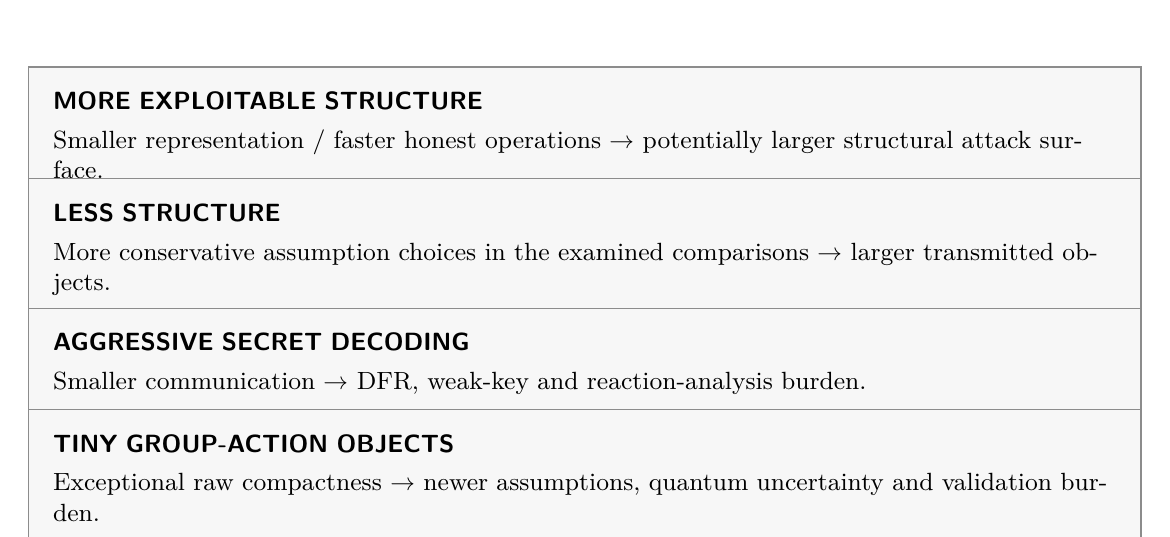
\begin{tikzpicture}[every node/.style={font=\small,align=left},box/.style={draw=black!45,fill=black!3,inner sep=9pt,text width=13.5cm}]
\node[box] (n0) at (0,0.0) {\textsf{\textbf{MORE EXPLOITABLE STRUCTURE}}\\[3pt]Smaller representation / faster honest operations $\rightarrow$ potentially larger structural attack surface.};
\node[box] (n1) at (0,-1.45) {\textsf{\textbf{LESS STRUCTURE}}\\[3pt]More conservative assumption choices in the examined comparisons $\rightarrow$ larger transmitted objects.};

\node[box] (n2) at (0,-2.9) {\textsf{\textbf{AGGRESSIVE SECRET DECODING}}\\[3pt]Smaller communication $\rightarrow$ DFR, weak-key and reaction-analysis burden.};

\node[box] (n3) at (0,-4.35) {\textsf{\textbf{TINY GROUP-ACTION OBJECTS}}\\[3pt]Exceptional raw compactness $\rightarrow$ newer assumptions, quantum uncertainty and validation burden.};

\end{tikzpicture}
\caption{Observed design pattern in the investigated families -- not a theorem. Rows are distinct mechanisms, not a universal monotonic law.}\label{fig:core}
\end{figure}

\hypertarget{why-no-new-kem-was-proposed}{%
\subsection{21. Why no new KEM was
proposed}\label{why-no-new-kem-was-proposed}}

Inventing a cipher to satisfy an output target would invite parameter
cherry-picking, concatenating unproved assumptions, overlooking DFR and
treating an unfamiliar group or tensor as proof of hardness. Each
apparent shortcut failed an immediate falsification: a two-byte DAWN
codec gain is engineering; HQC sparse supports are not transmitted;
BIKE-like removal of a codeword is already researched and
correctness-sensitive; historical 64 B CSIDH parameters have
quantum-resource controversy; MIKE's full CCA KEM and concrete quantum
story remain immature. Terminating these branches is the research
contribution. It prevents a construction with impressive bytes but a
missing security case.

\hypertarget{what-a-future-breakthrough-would-need}{%
\subsection{22. What a future breakthrough would
need}\label{what-a-future-breakthrough-would-need}}

A genuinely better KEM would need an efficiently samplable
\emph{average-case} public relation with a compact description, an
efficient secret-assisted recovery operation, no cheaply exploitable
symmetry or helper-data leakage, low/zero and preferably per-key bounded
failure, credible classical and fault-tolerant quantum resource
estimates, practical constant-time validation, low RAM/runtime, and a
clean IND-CCA reduction with measured complete objects. Worst-case
reductions would help where applicable, but only under distributions and
parameters that actually match the scheme. No investigated new problem
was shown to meet this conjunction. A mathematical advance could be a
new hard-instance distribution/decoder theorem, an unexpectedly tight
quantum bound for a non-regular action, or a compact CCA conversion
proven without costly auxiliary data; these are requirements, not
designs.

\hypertarget{open-questions}{%
\subsection{23. Open questions}\label{open-questions}}

Can a short public instance encode a secret-recoverable hard relation
without useful attacker symmetry? Can BIKE-like communication coexist
with a rigorous rare per-key DFR and reaction-resistant decoder? Can
DAWN's real correlated tail be bounded beyond the author's independence
model? What exactly changes in BAT's corrected game sequence? Can MIKE
gain independent concrete quantum cryptanalysis and an exact compact
IND-CCA/QROM construction? Can family-specific lower bounds relate
encoding, ciphertext correctness and attack structure? Can quantum ISD
and hidden-shift models be reconciled with hardware-relevant
depth/memory? See \texttt{OPEN\_RESEARCH\_QUESTIONS.md}.

\hypertarget{future-trigger-conditions}{%
\subsection{24. Future trigger
conditions}\label{future-trigger-conditions}}

Reopen only for new evidence that could change a specific gate:
independent MIKE security and complete CCA specification, a new
group-action quantum attack, canonical DAWN implementation/full-text
plus correlation-aware DFR bounds, the versioned BAT proof diff, a
rigorously bounded QC decoder at BIKE-like cost, major revised
lattice/ISD cost estimates, or a fundamentally new average-case problem
with an asymmetric recovery theorem. New NIST status alone affects
engineering guidance but does not retroactively prove a speculative
construction. \texttt{FUTURE\_TRIGGER\_CONDITIONS.md} assigns each
trigger to the affected conclusion.

\begin{longtable}[]{@{}
  >{\raggedright\arraybackslash}p{(\columnwidth - 4\tabcolsep) * \real{0.3333}}
  >{\raggedright\arraybackslash}p{(\columnwidth - 4\tabcolsep) * \real{0.3333}}
  >{\raggedright\arraybackslash}p{(\columnwidth - 4\tabcolsep) * \real{0.3333}}@{}}
\toprule\noalign{}
\begin{minipage}[b]{\linewidth}\raggedright
Trigger
\end{minipage} & \begin{minipage}[b]{\linewidth}\raggedright
Required evidence
\end{minipage} & \begin{minipage}[b]{\linewidth}\raggedright
Affected conclusion
\end{minipage} \\
\midrule\noalign{}
\endhead
\bottomrule\noalign{}
\endlastfoot
Independent MIKE quantum cryptanalysis & Exact sampler, independent
resource vectors and counteranalysis & Unknown concrete margin \\
Full MIKE IND-CCA KEM & Serialization, validation, reduction and losses,
independent implementation & Unknown complete KEM bytes / CCA path \\
New group-action quantum algorithm & Target-specific gates, depth, QRAM
and qubits & CSIDH / MIKE security ledger \\
Canonical DAWN implementation & Versioned algorithms and matched
reference vectors & Primary validation block \\
Correlation-aware DAWN DFR & Realistic per-key tail and
same-distribution analysis & Model versus real correctness \\
BAT proof-version comparison & Changed games, assumptions, losses and
parameter effects & Unknown correction impact \\
Rigorous BIKE-like per-key DFR & Extreme-tail theorem, reaction / CCA
analysis and matched performance & Secret-decoder obstacle \\
Major lattice attack changes & Comparable same-instance resource
estimates & Current lattice margins \\
Major quantum ISD changes & Comparable memory, depth and multi-target
model & QC security margins \\
New compact average-case hard problem & Sampled distribution, secret
recovery, quantum study and CCA bytes & Landscape rejection of
unsupported novelty \\
Verified McEliece structural attack & Separate distinguisher, heuristic
recovery and practical impact & McEliece qualification \\
NIST standardization change & Final normative text, parameters and
errata & Deployment status only \\
\end{longtable}

\hypertarget{limitations}{%
\subsection{25. Limitations}\label{limitations}}

\begin{center}\fbox{\begin{minipage}{.93\linewidth}
\textsf{\textbf{LIMITATIONS AT A GLANCE}}\par\smallskip
\small Canonical DAWN validation incomplete; BAT proof diff unresolved; DAWN DFR model reproduction is not an actual correlated DFR proof; no comprehensive independent lattice-estimator campaign; no physical quantum-computer experiment; MIKE concrete quantum margin unresolved; complete project-audited MIKE IND-CCA KEM unavailable; cross-platform RAM/runtime comparison incomplete.
\end{minipage}}\end{center}

The Phase 1 survey is targeted rather than exhaustive. Full primary
texts were inaccessible in some earlier phases, notably canonical DAWN
and version-paired BAT proof files. Phase 2A used a noncanonical
manuscript transcription for specific DAWN grouping and algebra; later
code reproduced its arithmetic, not official wire compatibility. An
author's DFR approximation was reproduced, not the real correlated
distribution. No full independently executed lattice estimator, quantum
ISD run, physical quantum hardware experiment, formal proof, or complete
measured RAM/stack comparison exists. The 2026 McEliece preprints
contain provable distinguisher and heuristic recovery claims of
different scope; neither is shown to practically break Classic
McEliece's deployed parameters here. MIKE's speed and proof statements
are author communications, not independently benchmarked complete CCA
KEM results. BAT's theorem-level correction is unknown, and concrete
MIKE quantum margin is unknown. These limits constrain the verdict; they
do not justify a positive construction by default.

\hypertarget{conclusion-and-engineering-recommendation}{%
\subsection{26. Conclusion and engineering
recommendation}\label{conclusion-and-engineering-recommendation}}

\textbf{No new KEM was identified as worth constructing under the
project's requirements.} Within the investigated design space and
evidence through 27 September 2026, no new mechanism combined a material
PK+CT gain, credible PQ security, adequate assumption maturity,
practical implementation and a defensible CCA path. The generalizable
result is a recurring compactness/security/maturity trade-off, not an
impossibility theorem and not proof that ML-KEM is optimal. For systems
requiring PQ key encapsulation now, use standardized, reviewed
constructions such as FIPS 203 ML-KEM, with normal protocol, validation
and side-channel controls;
\href{https://nvlpubs.nist.gov/nistpubs/FIPS/NIST.FIPS.203.pdf}{FIPS
203} recommends ML-KEM-768 as a default, while this paper often uses
ML-KEM-512 only as a level-1 size control. HQC is a selected code-based
diversification candidate in an ongoing standardization process; DAWN,
BAT, BIKE and group-action work retain their research qualifications.
The project's stop rule closes new-primitive construction until a
concrete trigger changes the evidence.

\begin{quote}
The investigation did not establish that substantially more compact
post-quantum KEMs are impossible. It established that, within the
examined design space and evidence available through 27 September 2026,
none of the investigated shortcuts justified constructing a new
primitive. Meaningful progress would require new mathematics or
substantially stronger evidence, not merely more aggressive parameters
or encoding.
\end{quote}

\clearpage

\hypertarget{references}{%
\subsection{References}\label{references}}

\begingroup\small\setstretch{1.0}

Publication type, version and evidence limits accompany each URL. A
paper's existence does not independently validate its concrete
parameters.

\hypertarget{standards-and-official-evaluations}{%
\subsubsection{Standards and official
evaluations}\label{standards-and-official-evaluations}}

\hypertarget{ref1}{}

\textbf{{[}1{]}} \textbf{NIST, STANDARD.} FIPS 203, ML-KEM
\url{https://csrc.nist.gov/pubs/fips/203/final}, 13 August 2024; exact
sizes, normative algorithms and status. A future erratum is noted.

\hypertarget{ref2}{}

\textbf{{[}2{]}} \textbf{NIST, OFFICIAL STATUS.} PQC project
\url{https://csrc.nist.gov/projects/post-quantum-cryptography}, updated
August 2026; HQC selected for ongoing standardization.

\hypertarget{ref3}{}

\textbf{{[}3{]}} \textbf{NIST, OFFICIAL EVALUATION.} IR 8545, Fourth
Round status
\url{https://nvlpubs.nist.gov/nistpubs/ir/2025/NIST.IR.8545.pdf}, March
2025; BIKE DFR concerns and HQC choice. Its older HQC size table is
superseded by the later team spec in this project.

\hypertarget{lattice-and-ntru}{%
\subsubsection{Lattice and NTRU}\label{lattice-and-ntru}}

\hypertarget{ref4}{}

\textbf{{[}4{]}} \textbf{Regev, PEER-REVIEWED.} On lattices, learning
with errors, random linear codes, and cryptography
\url{https://doi.org/10.1145/1060590.1060603}, STOC 2005. Reduction
context, not a proof for every concrete instance.

\hypertarget{ref5}{}

\textbf{{[}5{]}} \textbf{Langlois--Stehlé, EPRINT.} Module-lattice
reductions \url{https://eprint.iacr.org/2012/090}.

\hypertarget{ref6}{}

\textbf{{[}6{]}} \textbf{FrodoKEM authors, AUTHOR DRAFT.} CFRG draft-03
\url{https://datatracker.ietf.org/doc/draft-longa-cfrg-frodokem/}, June
2026; exact FrodoKEM-640 sizes.

\hypertarget{ref7}{}

\textbf{{[}7{]}} \textbf{NTRU team, AUTHOR SPEC.} Round-three
documentation \url{https://www.ntru.org/f/ntru-20190330.pdf}, HPS/HRSS
context.

\hypertarget{ref8}{}

\textbf{{[}8{]}} \textbf{NTRU Prime team, AUTHOR SPEC.} Round-three
documentation
\url{https://ntruprime.cr.yp.to/nist/ntruprime-20201007/Supporting_Documentation/doc.pdf}.

\hypertarget{ref9}{}

\textbf{{[}9{]}} \textbf{Liu et al., PEER-REVIEWED/EPRINT.} DAWN
\url{https://eprint.iacr.org/2025/1520}, ASIACRYPT 2025; ePrint revised
27 October 2025. Full canonical text inaccessible in project workflow;
abstract supports attributed size/assumption claims.

\hypertarget{ref10}{}

\textbf{{[}10{]}} \textbf{DAWN authors, AUTHOR REPOSITORY.} DFR
estimator \url{https://github.com/Icarid-Liu/lattice-KEM-DFR-estimator},
project-pinned commit 3c2602c30e13ce15ed7094ef97d9e4ed2dde01f6.
Arithmetic model, not encryption reference implementation.

\hypertarget{ref11}{}

\textbf{{[}11{]}} \textbf{Fouque et al., PEER-REVIEWED/EPRINT.} BAT
\url{https://eprint.iacr.org/2022/031}, TCHES 2022; ePrint revised 12
April 2026 with proof-error correction. Mathematical diff unverified.

\hypertarget{ref12}{}

\textbf{{[}12{]}} \textbf{CTRU/CNTR authors, EPRINT.} Compact and
Efficient KEMs over NTRU Lattices
\url{https://eprint.iacr.org/2022/579}.

\hypertarget{ref13}{}

\textbf{{[}13{]}} \textbf{NTRU+ team, AUTHOR SPEC.} NTRU+
\url{https://www.ntruplus.org/}; use version-specific claims only.

\hypertarget{ref14}{}

\textbf{{[}14{]}} \textbf{Hofheinz--Hövelmanns--Kiltz,
PEER-REVIEWED/EPRINT.} Modular analysis of Fujisaki--Okamoto
\url{https://eprint.iacr.org/2017/604}; transform hypotheses are not
automatically met by bare NIKE.

\hypertarget{codes-and-recent-structural-cryptanalysis}{%
\subsubsection{Codes and recent structural
cryptanalysis}\label{codes-and-recent-structural-cryptanalysis}}

\hypertarget{ref15}{}

\textbf{{[}15{]}} \textbf{HQC team, AUTHOR SPEC.} HQC, 22 August 2025
\url{https://pqc-hqc.org/doc/hqc_specifications_2025_08_22.pdf}, Tables
5--6; the project uses 2241/4433 B at level 1.

\hypertarget{ref16}{}

\textbf{{[}16{]}} \textbf{BIKE team, AUTHOR SPEC.} BIKE v5.2
\url{https://bikesuite.org/files/v5.2/BIKE_Spec.2024.10.10.1.pdf}, 10
October 2024. Full PDF timed out in the earlier audit; avoid unsupported
theorem attribution.

\hypertarget{ref17}{}

\textbf{{[}17{]}} \textbf{Open Quantum Safe, IMPLEMENTATION DOC.} BIKE
table \url{https://openquantumsafe.org/liboqs/algorithms/kem/bike.html},
L1 1541/1573 B; its page labels implemented spec v5.1 and IND-CPA.

\hypertarget{ref18}{}

\textbf{{[}18{]}} \textbf{Classic McEliece team, AUTHOR DOC.}
Implementation sizes \url{https://classic.mceliece.org/impl.html},
specification \url{https://classic.mceliece.org/spec.html}.

\hypertarget{ref19}{}

\textbf{{[}19{]}} \textbf{Annechini et al., EPRINT/CRYPTO 2026 line.}
QC-MDPC DFR \url{https://eprint.iacr.org/2025/1043}, an analytic decoder
model.

\hypertarget{ref20}{}

\textbf{{[}20{]}} \textbf{Ghoshal et al., EPRINT/PREPRINT.}
Quasipolynomial cryptanalysis of McEliece
\url{https://eprint.iacr.org/2026/1630}, revised 27 August 2026:
provable distinguisher and heuristic recovery extensions; concrete
attacks described as not yet practical.

\hypertarget{ref21}{}

\textbf{{[}21{]}} \textbf{Briaud et al., EPRINT/PREPRINT.} Heuristic
subexponential McEliece attack \url{https://eprint.iacr.org/2026/1232},
revised 17 September 2026: challenges and heuristic extrapolation, not a
practical Classic McEliece level-1 break.

\hypertarget{historical-failures-and-group-actions}{%
\subsubsection{Historical failures and group
actions}\label{historical-failures-and-group-actions}}

\hypertarget{ref22}{}

\textbf{{[}22{]}} \textbf{Castryck--Decru, PEER-REVIEWED/EPRINT.} SIDH
key recovery \url{https://eprint.iacr.org/2022/975}, EUROCRYPT 2023;
public torsion images essential.

\hypertarget{ref23}{}

\textbf{{[}23{]}} \textbf{Beullens, PEER-REVIEWED/EPRINT.} Breaking
Rainbow Takes a Weekend on a Laptop
\url{https://eprint.iacr.org/2022/214}, CRYPTO 2022.

\hypertarget{ref24}{}

\textbf{{[}24{]}} \textbf{Tao--Petzoldt--Ding, PEER-REVIEWED.} HFE
variant attacks
\url{https://csrc.nist.gov/CSRC/media/Events/third-pqc-standardization-conference/documents/accepted-papers/petzoldt-efficient-key-pqc2021.pdf},
CRYPTO 2021.

\hypertarget{ref25}{}

\textbf{{[}25{]}} \textbf{Shamir, PEER-REVIEWED.} Basic Merkle--Hellman
break
\url{https://www-igm.univ-mlv.fr/~jyt/Crypto/crack_merkle_hellman.pdf},
IEEE IT 1984.

\hypertarget{ref26}{}

\textbf{{[}26{]}} \textbf{Hart et al., EPRINT/PKC.} Practical
cryptanalysis of WalnutDSA \url{https://eprint.iacr.org/2017/1160}.

\hypertarget{ref27}{}

\textbf{{[}27{]}} \textbf{Castryck et al., PEER-REVIEWED/EPRINT.} CSIDH
\url{https://eprint.iacr.org/2018/383}, ASIACRYPT 2018; historical
compact exchange.

\hypertarget{ref28}{}

\textbf{{[}28{]}} \textbf{Bonnetain--Schrottenloher, PEER-REVIEWED.}
Quantum Security Analysis of CSIDH
\url{https://zhengxuisogeny.github.io/Isogeny-Based-Cryptography/index/quantumcsidh.pdf},
EUROCRYPT 2020, Table 4 and field-size tradeoffs.

\hypertarget{ref29}{}

\textbf{{[}29{]}} \textbf{CSIDH team, AUTHOR ANALYSIS.} Quantum-security
response \url{https://csidh.isogeny.org/analysis.html}; disputes oracle
estimates.

\hypertarget{ref30}{}

\textbf{{[}30{]}} \textbf{Frixons et al., EPRINT.} Shifted-input
vectorization quantum attack \url{https://eprint.iacr.org/2025/376.pdf},
2025; multiple public curves/QRAM.

\hypertarget{ref31}{}

\textbf{{[}31{]}} \textbf{Banegas et al., EPRINT.} dCTIDH
\url{https://eprint.iacr.org/2025/107.pdf}, 2025; platform-specific
cycles.

\hypertarget{ref32}{}

\textbf{{[}32{]}} \textbf{Banegas et al., PREPRINT.} Hardened CTIDH
\url{https://arxiv.org/abs/2509.12877}, 2025; dummy-free evaluation.

\hypertarget{ref33}{}

\textbf{{[}33{]}} \textbf{Robert, EPRINT/PREPRINT.} Module action
\url{https://eprint.iacr.org/2024/1556.pdf}, October 2024; mathematical
MIKE proposal.

\hypertarget{ref34}{}

\textbf{{[}34{]}} \textbf{Robert/MIKE team, AUTHOR ANNOUNCEMENT.} July
2026 mailing-list claims
\url{https://mailarchive.ietf.org/arch/msg/cfrg/QM3t6di1bsgla6iIJ3gN6BbDoVk/};
64 B, speed and algebraic-model claims, not independent full CCA
evidence.

\hypertarget{ref35}{}

\textbf{{[}35{]}} \textbf{Årdal--Basso--Riepel, PEER-REVIEWED/EPRINT.}
Algebraic Isogeny Model \url{https://eprint.iacr.org/2026/032},
EUROCRYPT 2026; model results are not automatically standard-model KEM
proofs.

\hypertarget{ref36}{}

\textbf{{[}36{]}} \textbf{Qi, PEER-REVIEWED.} CSIDH KEM / CSIKE
\url{https://doi.org/10.1515/jmc-2022-0007}, 2022; modern parameter and
QROM audit still needed.

\hypertarget{ref37}{}

\textbf{{[}37{]}} \textbf{Dartois et al., PEER-REVIEWED/EPRINT.} PEGASIS
\url{https://eprint.iacr.org/2025/401}, CRYPTO 2025.

\endgroup
\clearpage\begin{landscape}
\section{Appendix A. Byte accounting}
\small PK + CT means one recipient public key plus one complete ciphertext; bytes are not security scores. Raw group-action exchanges are excluded from the KEM CT and total columns. Unknown is not zero.\\[8pt]
\small\setlength{\tabcolsep}{4pt}\renewcommand{\arraystretch}{1.25}
\begin{longtable}{p{2.7cm}p{2.2cm}r r r p{3.7cm}p{7cm}}
\toprule System & Family & PK (B) & CT (B) & Sum (B) & Status & Qualification \\ \midrule
\endfirsthead
\toprule System & Family & PK (B) & CT (B) & Sum (B) & Status & Qualification \\ \midrule
\endhead
ML-KEM-512 & Module-LWE & 800 & 768 & 1568 & STANDARDIZED & FIPS 203; level-1 size control, not a universal PQ security number. \\
ML-KEM-768 & Module-LWE & 1184 & 1088 & 2272 & STANDARDIZED & FIPS 203 default recommendation. \\
FrodoKEM-640 & Plain LWE & 9616 & 9752 & 19368 & RESEARCH CONSTRUCTION & June 2026 draft-03; not eFrodo. \\
DAWN-alpha-512 & NTRU + Ring-LWE & 615 & 436 & 1051 & RESEARCH CONSTRUCTION & Author claim; grouped model reproduced; canonical validation incomplete. \\
DAWN-beta-512 & NTRU + Ring-LWE & 514 & 450 & 964 & RESEARCH CONSTRUCTION & Real DFR and independent estimator gate unresolved. \\
BAT-512 & NTRU short basis & 521 & 473 & 994 & HISTORICAL & Research comparison; 2026 proof correction diff UNKNOWN. \\
HQC-1 & QC Hamming & 2241 & 4433 & 6674 & SELECTED / STANDARDIZATION IN PROGRESS & 2025-08-22 spec; final HQC FIPS not claimed. \\
BIKE-1 & QC-MDPC & 1541 & 1573 & 3114 & RESEARCH CONSTRUCTION & OQS table: v5.1 / IND-CPA label; v5.2 transform claims separate. Nonselection is not a break. \\
Classic McEliece 348864 & Binary Goppa & 261120 & 96 & 261216 & RESEARCH CONSTRUCTION & No valid-input DFR; 2026 preprints not a demonstrated practical parameter break. \\
CSIDH-512 example & Class-group action & 64 raw & UNKNOWN & UNKNOWN & HISTORICAL & Peer curve 64 B; 128 B raw exchange. PQ128 disputed; CCA total unknown. \\
CSIDH enlarged examples & Class-group action & $\sim$283 / $\sim$660 raw & UNKNOWN & UNKNOWN & RESEARCH CONSTRUCTION & $\sim$2260 / $\sim$5280-bit model regimes: $\sim$566 / $\sim$1320 B raw pairs; not established CCA sets. \\
MIKE example & Hermitian-module action & 64 claimed & UNKNOWN & UNKNOWN & EMERGING RESEARCH & Peer $\sim$64 B inferred; $\sim$128 B raw exchange. Complete IND-CCA CT unknown. \\
\bottomrule\end{longtable}
\normalsize Source versions and qualifications: Sections 5, 9, 12--17 and bibliography items 1, 6, 9, 11, 15--18, 27--34. The grouped DAWN sizes are independently reproduced only within the project model.
\end{landscape}

\hypertarget{appendix-b.-attack-ledgers}{%
\subsection{Appendix B. Attack
ledgers}\label{appendix-b.-attack-ledgers}}

\begin{longtable}[]{@{}
  >{\raggedright\arraybackslash}p{(\columnwidth - 4\tabcolsep) * \real{0.3333}}
  >{\raggedright\arraybackslash}p{(\columnwidth - 4\tabcolsep) * \real{0.3333}}
  >{\raggedright\arraybackslash}p{(\columnwidth - 4\tabcolsep) * \real{0.3333}}@{}}
\toprule\noalign{}
\begin{minipage}[b]{\linewidth}\raggedright
Family
\end{minipage} & \begin{minipage}[b]{\linewidth}\raggedright
Examined attack surface
\end{minipage} & \begin{minipage}[b]{\linewidth}\raggedright
Project result / unresolved evidence
\end{minipage} \\
\midrule\noalign{}
\endhead
\bottomrule\noalign{}
\endlastfoot
NTRU & Short/equivalent relations; primal, dual and hybrid attacks;
automorphisms; CRT; ephemeral attacks & No fresh numerical estimator
run. Pinned lattice-estimator commit:
\nolinkurl{53da5982597709ba0fdf94ea37a84d822310fd84}; Sage unavailable
in the research phase. Ring factorization is not an attack. \\
QC Hamming & Classical/quantum ISD; rotations; sparse duals; weak keys;
failures and reactions & No new quantum ISD campaign. Secret-decoder
rare per-key tails remain central. \\
Regular group actions & Hidden shift; coherent oracle costs; memory/time
trade-offs; related-input attacks & CSIDH-512 modeled vectors appear in
Section 15; physical attack and agreed PQ128 interpretation were not
established. \\
MIKE & New module-action assumptions; quantum algorithms; domain
validation; CCA transform & Independent concrete quantum margin and
complete project-audited IND-CCA KEM remain UNKNOWN. \\
\end{longtable}

For CSIDH-512, the cited log2 vectors (queries, T gates, classical time,
quantum memory) are (33, 85.6, 33, 31), (19, 71.6, 86, \textless15.3),
and (24, 76.6, 63, \textless15.3). These include the paper's oracle
model and remain disputed in concrete accounting. Shifted-input results
require additional related curves and do not apply directly to ordinary
two-object CSIDH.

\hypertarget{appendix-c.-evidence-and-confidence}{%
\subsection{Appendix C. Evidence and
confidence}\label{appendix-c.-evidence-and-confidence}}

\begin{longtable}[]{@{}
  >{\raggedright\arraybackslash}p{(\columnwidth - 4\tabcolsep) * \real{0.3333}}
  >{\raggedright\arraybackslash}p{(\columnwidth - 4\tabcolsep) * \real{0.3333}}
  >{\raggedright\arraybackslash}p{(\columnwidth - 4\tabcolsep) * \real{0.3333}}@{}}
\toprule\noalign{}
\begin{minipage}[b]{\linewidth}\raggedright
Decisive claim
\end{minipage} & \begin{minipage}[b]{\linewidth}\raggedright
Evidence role / confidence
\end{minipage} & \begin{minipage}[b]{\linewidth}\raggedright
Boundary
\end{minipage} \\
\midrule\noalign{}
\endhead
\bottomrule\noalign{}
\endlastfoot
ML-KEM byte encodings / status & EXTERNAL LITERATURE RESULT /
ESTABLISHED & Conditional hardness; no optimality theorem. \\
DAWN grouped sizes and two-byte slack & PROJECT-DERIVED /
PROJECT-REPRODUCED & Model from transcription; no official wire-vector
validation. \\
DAWN log2 model outputs & PROJECT-DERIVED / PROJECT-REPRODUCED & Real
correlated and per-key DFR UNKNOWN. \\
BAT proof correction & EXTERNAL metadata / ESTABLISHED as revision &
Exact changed theorem and parameter effect UNKNOWN. \\
QC support entropy & PROJECT-DERIVED / PROJECT-REPRODUCED & Supports are
not transmitted; no public compression algorithm. \\
MIKE 64 B and speed & EXTERNAL / AUTHOR CLAIM & Matching independent
benchmark and full KEM audit absent. \\
MIKE roughly 128 B raw exchange & INFERENCE / PLAUSIBLE & Not complete
IND-CCA communication. \\
No new construction justified & PROJECT-DERIVED / STRONGLY SUPPORTED
scoped judgment & Not universal impossibility or a family-wide break. \\
\end{longtable}

\hypertarget{appendix-d.-reproduction-notes}{%
\subsection{Appendix D. Reproduction
notes}\label{appendix-d.-reproduction-notes}}

Publication rerun: Python 3.12.14, NumPy 2.3.5, Linux x86-64. All seven
original scripts were executed successfully. Three original codec unit
tests passed. No timing benchmark is inferred from this rerun.

The DFR source model was pinned to author repository commit
\texttt{3c2602c30e13ce15ed7094ef97d9e4ed2dde01f6}. Positive float64
convolution reproduces the specified independence model. It does not
supply the missing correlated, per-key or adversarial-input theorem.

Observed modeled log2 DFR: alpha −132.676946974; beta −130.133613254.
HQC-1 support entropy: secret 622.952 bits; ephemeral 694.542 bits.
BIKE-1 joint error support: 1196.018 bits. Ring calculation: 128
degree-four factors for each modulus, with 512 odd-power automorphisms.

From the repository root:

\begin{Shaded}
\begin{Highlighting}[]
\ExtensionTok{python} \AttributeTok{{-}m}\NormalTok{ pip install }\AttributeTok{{-}r}\NormalTok{ requirements.txt}
\ExtensionTok{python} \AttributeTok{{-}m}\NormalTok{ unittest discover }\AttributeTok{{-}s}\NormalTok{ experiments }\AttributeTok{{-}p} \StringTok{\textquotesingle{}test\_*.py\textquotesingle{}} \AttributeTok{{-}v}
\ExtensionTok{python}\NormalTok{ experiments/check\_reproduced\_results.py}
\end{Highlighting}
\end{Shaded}

The repository's REPRODUCIBILITY.md lists every script, exact command
and boundary. A green CI result means numerical/software reproduction
only.

\hypertarget{appendix-e.-falsified-mechanisms}{%
\subsection{Appendix E. Falsified
mechanisms}\label{appendix-e.-falsified-mechanisms}}

\begin{longtable}[]{@{}
  >{\raggedright\arraybackslash}p{(\columnwidth - 4\tabcolsep) * \real{0.3333}}
  >{\raggedright\arraybackslash}p{(\columnwidth - 4\tabcolsep) * \real{0.3333}}
  >{\raggedright\arraybackslash}p{(\columnwidth - 4\tabcolsep) * \real{0.3333}}@{}}
\toprule\noalign{}
\begin{minipage}[b]{\linewidth}\raggedright
Mechanism
\end{minipage} & \begin{minipage}[b]{\linewidth}\raggedright
Falsification / stopping reason
\end{minipage} & \begin{minipage}[b]{\linewidth}\raggedright
Scope
\end{minipage} \\
\midrule\noalign{}
\endhead
\bottomrule\noalign{}
\endlastfoot
Ordinary DAWN packing improvement & Same-alphabet slack is 2 B, about
0.2075\%; does not meet a 5\% gate & Larger mathematical changes remain
open. \\
Send sparse-error seeds & Reveals the error or secret-dependent preimage
& Does not supply a secure public compressor. \\
Replace HQC dense objects with message/salt & Discloses the KEM preimage
& Shannon entropy alone is not efficient cryptographic encoding. \\
Delete HQC's noisy codeword & Returns to existing private-decoder
territory and rare-tail burden & Not a lower bound on all code KEMs. \\
Treat 64 B CSIDH as proven PQ128 CCA & Ignores resource-model
controversy and full transform overhead & Regular-action research is not
declared insecure. \\
Promote MIKE raw exchange to full KEM & Complete ciphertext, independent
quantum margin and CCA evidence absent & Promising research signal, not
a break claim. \\
\end{longtable}

\hypertarget{appendix-f.-reproducibility-code-overview}{%
\subsection{Appendix F. Reproducibility code
overview}\label{appendix-f.-reproducibility-code-overview}}

All paths below are relative to the repository root. Every script exists
in the accompanying package. Constants are embedded, so the documented
commands require no downloaded research inputs.

\begin{longtable}[]{@{}
  >{\raggedright\arraybackslash}p{(\columnwidth - 4\tabcolsep) * \real{0.3333}}
  >{\raggedright\arraybackslash}p{(\columnwidth - 4\tabcolsep) * \real{0.3333}}
  >{\raggedright\arraybackslash}p{(\columnwidth - 4\tabcolsep) * \real{0.3333}}@{}}
\toprule\noalign{}
\begin{minipage}[b]{\linewidth}\raggedright
Filename in experiments/
\end{minipage} & \begin{minipage}[b]{\linewidth}\raggedright
Inputs and outputs
\end{minipage} & \begin{minipage}[b]{\linewidth}\raggedright
Reproduces / does not establish
\end{minipage} \\
\midrule\noalign{}
\endhead
\bottomrule\noalign{}
\endlastfoot
dawn\_codec.py & 512 coefficients; four radix/group formats → grouped
and whole-vector byte ledger & Modeled packing and bijection; no
official wire compatibility, KEM correctness or security. \\
test\_dawn\_codec.py & Seeded vectors, boundaries and malformed inputs →
three unit tests & Local codec round trips/rejection; no production
hardening or security proof. \\
reproduce\_dawn\_dfr\_model.py & Author-model parameters →
positive-convolution log2 tails & Specified arithmetic; no actual
correlated or per-key DFR. \\
paired\_noise\_check.py & Restricted iid model at n = 512 →
joint/marginal tail ratios & Paired-surrogate dependence; no corrected
DAWN DFR. \\
toy\_correlation.py & n = 8, one +1 and one −1 → exhaustive 3136-pair
histogram & Toy dependence counterexample; not full DAWN parameters. \\
ring\_structure.py & q = 257, 769; polynomial identities → factor
degrees and counts & Algebraic identities; no lattice key-recovery
advantage. \\
qc\_entropy\_frontier.py & HQC/BIKE weights and dimensions → binomial
entropy and bytes & Representation accounting; no public compressor,
attack estimate or DFR proof. \\
check\_reproduced\_results.py & Known expected values → assertions &
Publication regression checks only; no cryptographic security
validation. \\
\end{longtable}

\hypertarget{selected-code-listings}{%
\subsubsection{Selected code listings}\label{selected-code-listings}}

\textbf{Listing 1 --- experiments/dawn\_codec.py.} Exact whole-alphabet
byte bound. This does not establish official serialization compatibility
or KEM security.

\begin{Shaded}
\begin{Highlighting}[]
\KeywordTok{def}\NormalTok{ theoretical\_bytes(fmt: Format) }\OperatorTok{{-}\textgreater{}} \BuiltInTok{int}\NormalTok{:}
    \ControlFlowTok{return}\NormalTok{ ((fmt.alphabet}\OperatorTok{**}\NormalTok{N }\OperatorTok{{-}} \DecValTok{1}\NormalTok{).bit\_length() }\OperatorTok{+} \DecValTok{7}\NormalTok{) }\OperatorTok{//} \DecValTok{8}
\end{Highlighting}
\end{Shaded}

\textbf{Listing 2 --- experiments/reproduce\_dawn\_dfr\_model.py.}
Positive convolution of an assumed independent kernel. The assumption is
an input, not an experimental conclusion.

\begin{Shaded}
\begin{Highlighting}[]
\NormalTok{a, a0 }\OperatorTok{=}\NormalTok{ vector(kernel)}
\NormalTok{dist }\OperatorTok{=}\NormalTok{ np.array([}\FloatTok{1.0}\NormalTok{])}\OperatorTok{;}\NormalTok{ lo }\OperatorTok{=} \DecValTok{0}
\ControlFlowTok{for}\NormalTok{ \_ }\KeywordTok{in} \BuiltInTok{range}\NormalTok{(n):}
\NormalTok{    dist }\OperatorTok{=}\NormalTok{ np.convolve(dist, a)}
\NormalTok{    lo }\OperatorTok{+=}\NormalTok{ a0}
\end{Highlighting}
\end{Shaded}

\textbf{Listing 3 --- experiments/qc\_entropy\_frontier.py.}
Fixed-weight support entropy. This support is not the transmitted dense
object and provides no direct bandwidth saving.

\begin{Shaded}
\begin{Highlighting}[]
\KeywordTok{def}\NormalTok{ support\_bits(n, w):}
    \ControlFlowTok{return}\NormalTok{ log2(comb(n, w))}
\end{Highlighting}
\end{Shaded}


\end{document}
